\documentclass[aspectratio=169]{beamer}
\usepackage{amsmath}
\usepackage{amssymb}
\usepackage{tikz}
\usepackage{wasysym}
\usepackage{tikzsymbols}
\usepackage{xcolor}
\usepackage{animate}     % Option 1: play a PNG frame sequence
\usepackage{multimedia}  % Option 2: embed a video file (needs -shell-escape)
\usetikzlibrary{shapes,backgrounds,patterns}

% --- added for these slides -------------------------------------------------
\usepackage{pgfplots}
\pgfplotsset{compat=1.18, legend cell align=left}
\usetikzlibrary{arrows.meta,decorations.pathreplacing,calc,positioning}
\usepackage{listings}
\usepackage{booktabs}
% ----------------------------------------------------------------------------

% royalblue isn't a base xcolor name, so define it first (this is the default accent)
\definecolor{royalblue}{RGB}{65,105,225}

% ============================================================
%  ACCENT COLOR: change ONE line below to switch the theme
%  Choose one of: royalblue , red , black
% ============================================================
\colorlet{accent}{royalblue}
% \colorlet{accent}{red}
% \colorlet{accent}{black}
% ============================================================

% Use default theme with white background
\usetheme{default}

% Make everything white/black, with the chosen accent color for structure
\setbeamercolor{background canvas}{bg=white}
\setbeamercolor{normal text}{fg=black}
\setbeamercolor{structure}{fg=accent}
\setbeamercolor{frametitle}{fg=accent,bg=white}
\setbeamercolor{title}{fg=accent}
\setbeamercolor{section in toc}{fg=black}
\setbeamercolor{block title}{fg=black,bg=gray!10}
\setbeamercolor{block body}{fg=black,bg=gray!5}
\setbeamercolor{block title example}{fg=black,bg=green!10}
\setbeamercolor{block body example}{fg=black,bg=green!5}
\setbeamercolor{block title alerted}{fg=black,bg=red!10}
\setbeamercolor{block body alerted}{fg=black,bg=red!5}

\usepackage{scalerel}

\newcommand{\subsmall}[1]{_{\scaleto{#1}{4pt}}}
\newcommand{\supsmall}[1]{^{\scaleto{#1}{2pt}}}

% Remove navigation symbols
\setbeamertemplate{navigation symbols}{}

% Simple footline with page numbers (single definition)
\setbeamertemplate{footline}{
    \hfill\makebox[5pt]{%
        \scriptsize\insertframenumber}
    \hspace*{2em}
    \vspace{0.5cm}
}

% Custom command for colored boxes
\newcommand{\cbox}[2]{\colorbox{#1}{\ensuremath{\displaystyle #2}}}

% --- code listings (Python), coloured with the accent -----------------------
\lstdefinestyle{py}{
  language=Python,
  basicstyle=\ttfamily\footnotesize,
  keywordstyle=\color{accent}\bfseries,
  commentstyle=\color{gray}\itshape,
  stringstyle=\color{green!45!black},
  showstringspaces=false,
  columns=fullflexible,
  keepspaces=true,
  backgroundcolor=\color{gray!6},
  frame=single, rulecolor=\color{gray!30},
  xleftmargin=2pt, xrightmargin=2pt,
  escapeinside={(*}{*)}
}
\lstset{style=py}

% --- shared plot style for the three "bound" pictures ------------------------
\pgfplotsset{
  boundplot/.style={
    width=5.9cm, height=4.6cm,
    axis lines=left, xmin=0, xmax=10, ymin=0, ymax=12,
    xtick=\empty, ytick=\empty,
    xlabel={$n$}, ylabel={time},
    every axis x label/.style={at={(axis description cs:1,0)},anchor=north east},
    every axis y label/.style={at={(axis description cs:0,1)},anchor=south east},
    samples=160, thick, clip mode=individual
  }
}

\title{Computational Complexity, Floating Point \& Convergence}
\subtitle{How fast, how accurate, how close?}
\author{Sharareh Sayyad}
\institute{Washington State University}
\date{January 30, 2026}

\begin{document}

% Title Slide
\frame{\titlepage}

% Table of Contents
\begin{frame}{Outline}
\tableofcontents
\end{frame}

% ============================================================
\section{Computational complexity and Big-$O$}
% ============================================================

\begin{frame}{What is computational complexity?}
\begin{columns}[c]
\begin{column}{0.5\textwidth}
\small
The \textbf{computational complexity} of an algorithm is the amount of
\textbf{resources} it needs, written as a function of the \textbf{input size} $n$.

\vspace{0.2cm}
Two resources matter most:
\begin{itemize}
  \item \textbf{Time complexity:} how many \textbf{flops} it performs.
        A \emph{flop} is one floating point operation: $+,\ -,\ \times,\ \div$.
  \item \textbf{Space complexity:} how much \emph{extra} memory it needs,
        beyond the input itself.
\end{itemize}
%\vspace{0.1cm}
%\begin{block}{Input size $n$}
%the length of a list, the number of digits of a number, the number of cities on a map, \dots
%\end{block}
\end{column}
\begin{column}{0.48\textwidth}
\centering
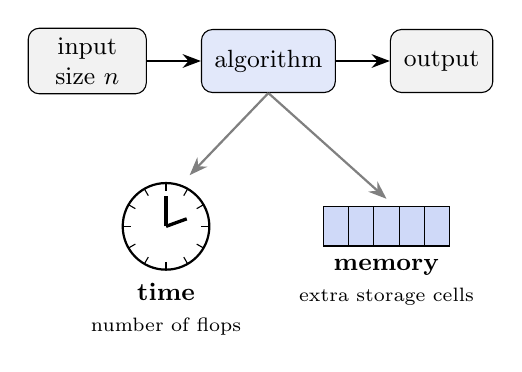
\begin{tikzpicture}[font=\small, >=Stealth]
  % input -> algorithm -> output
  \node[draw, rounded corners, fill=gray!10, minimum width=1.5cm, minimum height=0.8cm, align=center] (in) at (0,0) {input\\ size $n$};
  \node[draw, rounded corners, fill=accent!15, minimum width=1.7cm, minimum height=0.8cm] (alg) at (2.3,0) {algorithm};
  \node[draw, rounded corners, fill=gray!10, minimum width=1.3cm, minimum height=0.8cm] (out) at (4.5,0) {output};
  \draw[->, thick] (in) -- (alg);
  \draw[->, thick] (alg) -- (out);
  % time: a clock
  \begin{scope}[shift={(1.0,-2.1)}]
    \draw[thick, fill=white] (0,0) circle (0.55);
    \foreach \a in {0,30,...,330} \draw (\a:0.45) -- (\a:0.55);
    \draw[very thick] (0,0) -- (90:0.38);
    \draw[very thick] (0,0) -- (20:0.28);
    \node[below=0.6cm, align=center] at (0,0) {\textbf{time}\\ \scriptsize number of flops};
  \end{scope}
  % memory: a row of cells
  \begin{scope}[shift={(3.0,-2.35)}]
    \foreach \i in {0,...,4} \draw[fill=accent!25] (\i*0.32,0) rectangle ++(0.32,0.5);
    \node[below=0.05cm, align=center] at (0.8,0) {\textbf{memory}\\ \scriptsize extra storage cells};
  \end{scope}
  \draw[->, thick, gray] (alg.south) -- (1.3,-1.45);
  \draw[->, thick, gray] (alg.south) -- (3.8,-1.75);
\end{tikzpicture}
\end{column}
\end{columns}
\end{frame}

\begin{frame}[fragile]{Counting flops: the function $f(n)$}
\begin{columns}[T]
\begin{column}{0.52\textwidth}
\small
Count the flops of a function that computes the mean of a list of length $n$:
\begin{lstlisting}
def mean(x):
    s = 0.0           # 0 flops
    for a in x:       # n times:
        s = s + a     #  1 flop
    return s/len(x)   # 1 flop
\end{lstlisting}
\[
f(n) = \underbrace{n}_{\text{additions}} + \underbrace{1}_{\text{division}} = n + 1
\]
\begin{itemize}
  \item \textbf{Time:} $f(n) = n + 1$ flops.
  \item \textbf{Memory:} one extra variable \texttt{s}, whatever $n$ is.
\end{itemize}
\scriptsize Assignments, comparisons and the loop counter are not flops.
\end{column}
\begin{column}{0.45\textwidth}
\centering
\begin{tabular}{rr}
\toprule
$n$ & flops $f(n)$ \\
\midrule
10       & 11 \\
100      & 101 \\
1\,000   & 1\,001 \\
1\,000\,000 & 1\,000\,001 \\
\bottomrule
\end{tabular}
\vspace{0.3cm}
\begin{exampleblock}{Observation}
For large $n$ the ``$+1$'' hardly matters.
What matters is \emph{how $f(n)$ grows}: double $n$, double the flops.
\end{exampleblock}
\end{column}
\end{columns}
\end{frame}

\begin{frame}{Big-$O$: an upper bound on growth}
\begin{columns}[c]
\begin{column}{0.5\textwidth}
\small
\begin{block}{Definition}
$f(n) = O(g(n))$ if there are constants $c>0$ and $n_0$ with
\[
f(n) \le c\,g(n) \quad \text{for all } n \ge n_0 .
\]
\end{block}
\begin{itemize}
  \item ``$f$ grows no faster than $g$''.
  \item Drop constants and smaller terms:\\ $3n^2 + 10n + 50 = O(n^2)$.
\end{itemize}
\vspace{0.1cm}
\textbf{Two relatives}, briefly:\\[2pt]
\begin{tabular}{ll}
$\Omega(g)$ & lower bound: $f(n) \ge c\,g(n)$ \\
$\Theta(g)$ & tight: both $O(g)$ and $\Omega(g)$ \\
\end{tabular}
\end{column}
\begin{column}{0.48\textwidth}
\centering
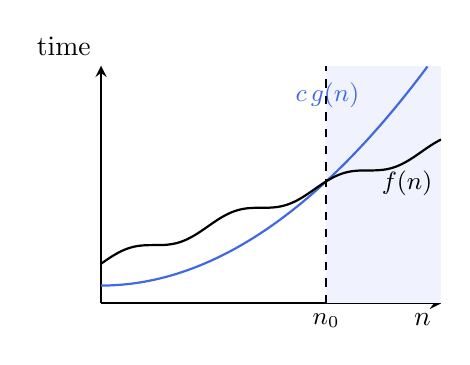
\begin{tikzpicture}
\begin{axis}[boundplot]
  \fill[accent!8] (axis cs:6.62,0) rectangle (axis cs:10,12);
  \addplot[accent, domain=0:9.6] {0.9+0.12*x^2};
  \addplot[black, domain=0:10] {2+0.6*x+0.3*sin(deg(2*x))};
  \node[accent, font=\small, left] at (axis cs:7.9,10.5) {$c\,g(n)$};
  \node[font=\small, below] at (axis cs:9,7.2) {$f(n)$};
  \draw[dashed] (axis cs:6.62,0) -- (axis cs:6.62,12);
  \node[below, font=\small] at (axis cs:6.62,0) {$n_0$};
\end{axis}
\end{tikzpicture}\\[4pt]
\scriptsize After $n_0$, $f$ stays below $c\,g$.
\end{column}
\end{columns}
\end{frame}

\begin{frame}{Big-$O$ in practice: reading loops}
\begin{columns}[T]
\begin{column}{0.53\textwidth}
\small
Count how many times the loop body runs, then keep the biggest term and drop constants.

\vspace{0.2cm}
\footnotesize
\begin{tabular}{@{}llc@{}}
\toprule
loop pattern & rounds & cost \\
\midrule
fixed number (e.g.\ 10) & $10$ & $O(1)$ \\
\texttt{i += c} up to $n$ & $n/c$ & $O(n)$ \\
\texttt{i *= 2} up to $n$ & $\log_2 n$ & $O(\log n)$ \\
two nested loops to $n$ & $n \cdot n$ & $O(n^2)$ \\
loop, then another loop & $n + n$ & $O(n)$ \\
\bottomrule
\end{tabular}

\vspace{0.3cm}
\begin{block}{Two rules}
\footnotesize
\textbf{Nested} loops \textbf{multiply}; loops \textbf{one after another} \textbf{add}.\\[2pt]
Example: a double loop, then a single loop: $n^2 + n = O(n^2)$.
\end{block}
\end{column}

\begin{column}{0.44\textwidth}
\centering
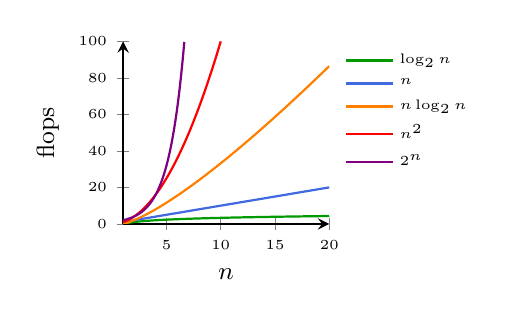
\begin{tikzpicture}
\begin{axis}[
  width=4.2cm, height=3.9cm, axis lines=left, xmin=1, xmax=20, ymin=0, ymax=100,
  xlabel={$n$}, ylabel={flops},
  legend style={font=\tiny, at={(1.03,1)}, anchor=north west, draw=none},
  samples=100, thick, tick label style={font=\tiny}, label style={font=\small}]
  \addplot[green!60!black, domain=1:20] {ln(x)/ln(2)}; \addlegendentry{$\log_2 n$}
  \addplot[accent, domain=1:20] {x};               \addlegendentry{$n$}
  \addplot[orange, domain=1:20] {x*ln(x)/ln(2)};   \addlegendentry{$n\log_2 n$}
  \addplot[red, domain=1:10] {x^2};                \addlegendentry{$n^2$}
  \addplot[violet, domain=1:6.64] {2^x};           \addlegendentry{$2^n$}
\end{axis}
\end{tikzpicture}

\vspace{0.1cm}
\begin{block}{The doubling test}
\scriptsize
Double $n$, watch the flop count:\\
$\times2 \Rightarrow O(n)$, \ $\times4 \Rightarrow O(n^2)$, \ $\times8 \Rightarrow O(n^3)$, \ $+1 \Rightarrow O(\log n)$.
\end{block}

\vspace{0.1cm}
\scriptsize Big-$O$ also describes \textbf{errors}: later we write error $= O(1/n)$ or $O(0.67^n)$.
\end{column}
\end{columns}
\end{frame}

% ============================================================
\section{Floating point numbers}
% ============================================================

\begin{frame}[fragile]{A computer cannot store every real number}
\begin{columns}[T]
\begin{column}{0.5\textwidth}
\small
\begin{lstlisting}
>>> 0.1 + 0.2
0.30000000000000004
>>> 0.1 + 0.2 == 0.3
False
\end{lstlisting}
\begin{itemize}
  \item A number is stored in a \textbf{fixed number of bits} (64 for a Python \texttt{float}).
  \item Only finitely many numbers fit, so most real numbers are \textbf{rounded} to the nearest one that does.
  \item $0.1$ has no exact binary form, just as $1/3 = 0.333\ldots$ has no exact decimal form.
\end{itemize}
\end{column}
\begin{column}{0.47\textwidth}
\centering
\small $0.1$ in binary repeats forever:\\[4pt]
$0.1 = 0.0\,0011\,0011\,0011\,0011\ldots_2$\\[10pt]
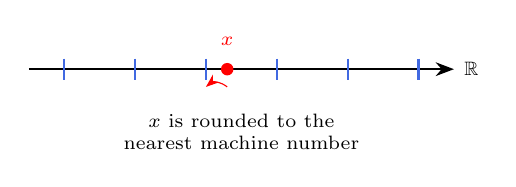
\begin{tikzpicture}[scale=0.9]
  \draw[thick, -{Stealth}] (0,0) -- (6,0) node[right]{\scriptsize $\mathbb{R}$};
  \foreach \x in {0.5,1.5,...,5.5} \draw[accent, thick] (\x,0.15) -- (\x,-0.15);
  \fill[red] (2.8,0) circle (2.5pt);
  \node[red, above, font=\scriptsize] at (2.8,0.2) {$x$};
  \draw[red, -{Stealth}] (2.8,-0.25) to[bend right=40] (2.5,-0.25);
  \node[below, font=\scriptsize, align=center] at (3,-0.5) {$x$ is rounded to the\\nearest machine number};
\end{tikzpicture}
\end{column}
\end{columns}
\end{frame}

\begin{frame}{Scientific notation}
\begin{columns}[T]
\begin{column}{0.56\textwidth}
\small
Write a number as
\[
x = \pm\, m \times 10^{\,e}, \qquad 1 \le m < 10
\]
\begin{itemize}
  \item $m$, the \textbf{mantissa}, holds the digits;
  \item $e$, the \textbf{exponent}, is an integer giving the size.
\end{itemize}
The digits of $m$ are the \textbf{significant digits}.
\end{column}
\begin{column}{0.4\textwidth}
\centering
\small Why ``floating point''?\\[4pt]
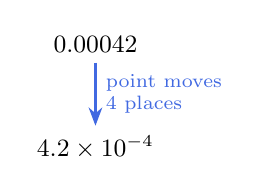
\begin{tikzpicture}[font=\small]
  \node (a) at (0,1.3) {$0.00042$};
  \node (b) at (0,0) {$4.2 \times 10^{-4}$};
  \draw[-{Stealth}, thick, accent] (a) -- (b) node[midway, right, font=\scriptsize, align=left] {point moves\\4 places};
\end{tikzpicture}\\[4pt]
\scriptsize The point \textbf{floats} to just after the first nonzero digit; the exponent remembers where it was.
\end{column}
\end{columns}
\vspace{0.3cm}
\centering
\small
\begin{tabular}{lccc}
\toprule
number & $299\,792\,458$ & $0.00042$ & $-1500$ \\
scientific & $2.99792458 \times 10^{8}$ & $4.2 \times 10^{-4}$ & $-1.5 \times 10^{3}$ \\
Python & \texttt{2.99792458e8} & \texttt{4.2e-4} & \texttt{-1.5e3} \\
significant digits & 9 & 2 & 2 \\
\bottomrule
\end{tabular}\\[6pt]
\scriptsize Huge and tiny numbers use the \emph{same} number of digits: precision is \textbf{relative} to the size.
\end{frame}

\begin{frame}{A toy computer with 3 significant digits}
\begin{columns}[T]
\begin{column}{0.47\textwidth}
\small
Store every number as $\pm\, d.dd \times 10^{\,e}$, with $-9 \le e \le 9$.
\begin{itemize}\footnotesize
  \item \textbf{Rounding:} $1/3 \to 3.33\times10^{-1}$, \ $2/3 \to 6.67\times10^{-1}$.
  \item \textbf{Gaps grow:} between 1 and 10 the gap is $0.01$, between 10 and 100 it is $0.1$, between 100 and 1000 it is $1$.
  \item \textbf{Relative error} of rounding: at most $\tfrac12\times10^{-2}$ ($0.5\%$), for every size.
  \item \textbf{Range:} largest $9.99\times10^{9}$, smallest positive $1.00\times10^{-9}$; beyond that, overflow and underflow.
\end{itemize}
\end{column}
\begin{column}{0.5\textwidth}
\centering
\small The same idea on a real computer:\\[4pt]
\scriptsize
\setlength{\tabcolsep}{3pt}
\begin{tabular}{lcc}
\toprule
 & toy & double \\
\midrule
base & 10 & 2 \\
mantissa & 3 digits & 53 bits \\
decimal digits & 3 & $\approx 16$ \\
rel.\ error & $5\times10^{-3}$ & $1.1\times10^{-16}$ \\
exponent & $[-9,\ 9]$ & $[-1022,\ 1023]$ \\
\bottomrule
\end{tabular}\\[8pt]
\begin{alertblock}{Key idea}
\scriptsize Floating point = scientific notation with a \textbf{fixed number of digits}. Gaps, $\varepsilon$ and rounding all come from this, in base 2.
\end{alertblock}
\end{column}
\end{columns}
\end{frame}

\begin{frame}{The floating point format}
Scientific notation in base 2, with a fixed number of bits:
\[
x = \pm\, (1.f_1 f_2 \ldots f_{52})_2 \times 2^{\,e}
\]
\centering
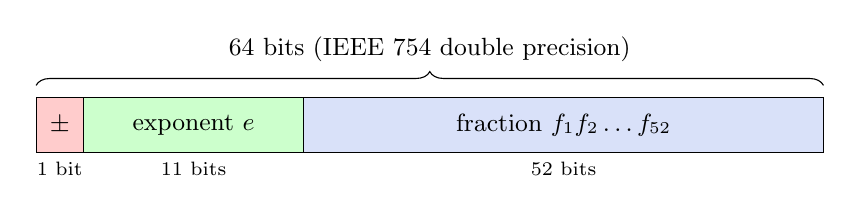
\begin{tikzpicture}[font=\small]
  \draw[fill=red!20]   (0,0) rectangle (0.6,0.7);   \node at (0.3,0.35) {$\pm$};
  \draw[fill=green!20] (0.6,0) rectangle (3.4,0.7); \node at (2.0,0.35) {exponent $e$};
  \draw[fill=accent!20] (3.4,0) rectangle (10,0.7); \node at (6.7,0.35) {fraction $f_1 f_2 \ldots f_{52}$};
  \node[below, font=\scriptsize] at (0.3,0) {1 bit};
  \node[below, font=\scriptsize] at (2.0,0) {11 bits};
  \node[below, font=\scriptsize] at (6.7,0) {52 bits};
  \draw[decorate, decoration={brace, amplitude=5pt}] (0,0.85) -- (10,0.85) node[midway, above=5pt] {64 bits (IEEE 754 double precision)};
\end{tikzpicture}

\vspace{0.4cm}
\begin{columns}[T]
\begin{column}{0.48\textwidth}
\begin{block}{Fraction (52 bits)}
\small decides the \textbf{precision}: about 16 significant decimal digits.
\end{block}
\end{column}
\begin{column}{0.48\textwidth}
\begin{block}{Exponent (11 bits)}
\small decides the \textbf{range}: from about $10^{-308}$ to $10^{308}$.
\end{block}
\end{column}
\end{columns}
\end{frame}

\begin{frame}{The number line has gaps, and they grow}
\begin{columns}[c]
\begin{column}{0.5\textwidth}
\small
\begin{itemize}
  \item Between two powers of 2 the machine numbers are \textbf{evenly spaced}.
  \item Each time we pass a power of 2, the spacing \textbf{doubles}.
  \item So the \emph{relative} spacing stays about the same everywhere.
\end{itemize}
\vspace{0.2cm}
\centering
\begin{tabular}{rr}
\toprule
$x$ & gap to the next float \\
\midrule
$1$ & $2.2\times10^{-16}$ \\
$10^{8}$ & $1.5\times10^{-8}$ \\
$10^{16}$ & $2$ \\
\bottomrule
\end{tabular}\\[3pt]
\scriptsize (\texttt{np.spacing(x)}) \quad so \texttt{1e16 + 1 == 1e16} is \texttt{True}!
\end{column}
\begin{column}{0.47\textwidth}
\centering
\small a toy system with 2 fraction bits\\[4pt]
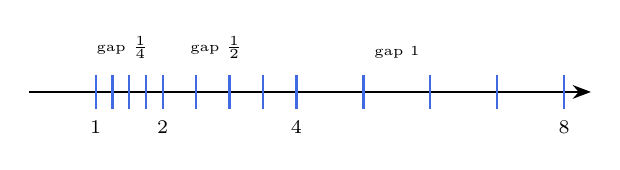
\begin{tikzpicture}[xscale=0.85, yscale=1.2]
  \draw[thick, -{Stealth}] (0,0) -- (8.4,0);
  \foreach \x in {1,1.25,1.5,1.75} \draw[accent, thick] (\x,0.18) -- (\x,-0.18);
  \foreach \x in {2,2.5,3,3.5} \draw[accent, thick] (\x,0.18) -- (\x,-0.18);
  \foreach \x in {4,5,6,7} \draw[accent, thick] (\x,0.18) -- (\x,-0.18);
  \draw[accent, thick] (8,0.18) -- (8,-0.18);
  \foreach \x in {1,2,4,8} \node[below, font=\scriptsize] at (\x,-0.2) {\x};
  \node[above, font=\tiny] at (1.4,0.25) {gap $\tfrac14$};
  \node[above, font=\tiny] at (2.8,0.25) {gap $\tfrac12$};
  \node[above, font=\tiny] at (5.5,0.25) {gap $1$};
\end{tikzpicture}
\end{column}
\end{columns}
\end{frame}

\begin{frame}{Machine epsilon and rounding error}
\begin{columns}[T]
\begin{column}{0.52\textwidth}
\begin{block}{Machine epsilon}
$\varepsilon = 2^{-52} \approx 2.2 \times 10^{-16}$, the gap between $1$ and the next float.\\[2pt]
\small (\texttt{np.finfo(float).eps})
\end{block}
\begin{block}{Rounding}
Storing $x$ gives $\mathrm{fl}(x) = x(1+\delta)$ with $|\delta| \le \varepsilon/2$.
\end{block}
\small Every flop ($+,-,\times,/$) is computed exactly, then rounded: a \textbf{relative} error of at most $\varepsilon/2$ each time.
\end{column}
\begin{column}{0.45\textwidth}
\begin{exampleblock}{Rule of thumb}
\small A double carries about \textbf{16 significant digits}. Asking for more accuracy than $\approx10^{-16}$ (relative) is asking for the impossible.
\end{exampleblock}
\vspace{0.2cm}
\small Finding $\varepsilon$ yourself:
\begin{center}
\texttt{eps ← 1}\\
\texttt{while 1 + eps/2 > 1:}\\
\texttt{\ \ \ \ eps ← eps/2}
\end{center}
\scriptsize (Problem 2 in the notebook)
\end{column}
\end{columns}
\end{frame}

\begin{frame}{Range: overflow, underflow, \texttt{inf} and \texttt{nan}}
\centering
\small
\begin{tabular}{lll}
\toprule
situation & example & result \\
\midrule
largest float & \texttt{np.finfo(float).max} & $\approx 1.8\times10^{308}$ \\
overflow & \texttt{1e308 * 10} & \texttt{inf} \\
smallest normal float & \texttt{np.finfo(float).tiny} & $\approx 2.2\times10^{-308}$ \\
underflow & \texttt{1e-308 / 1e100} & \texttt{0.0} \\
undefined & \texttt{inf - inf},\ \ \texttt{0 * inf} & \texttt{nan} (not a number) \\
\bottomrule
\end{tabular}

\vspace{0.4cm}
\begin{alertblock}{Watch out}
\texttt{nan} spreads: any calculation with a \texttt{nan} gives \texttt{nan}, and \texttt{nan == nan} is \texttt{False}. Use \texttt{np.isnan(x)} to test for it.
\end{alertblock}
\end{frame}

\begin{frame}[fragile]{Pitfall 1: comparing and adding floats}
\begin{columns}[T]
\begin{column}{0.48\textwidth}
\textbf{Never test floats with \texttt{==}}
\begin{lstlisting}
x = 0.1 + 0.2
x == 0.3              # False
abs(x - 0.3) < 1e-12  # True
np.isclose(x, 0.3)    # True
\end{lstlisting}
\small Compare with a \textbf{tolerance}.
\end{column}
\begin{column}{0.48\textwidth}
\textbf{Small plus large loses the small}
\begin{lstlisting}
1e16 + 1 - 1e16  # 0.0
1e16 - 1e16 + 1  # 1.0
\end{lstlisting}
\small The order of operations matters: floating point addition is \textbf{not associative}.\\[4pt]
Summing many small numbers into a big total slowly loses digits.
\end{column}
\end{columns}
\end{frame}

\begin{frame}{Pitfall 2: catastrophic cancellation}
\begin{columns}[c]
\begin{column}{0.48\textwidth}
\small
Subtracting two \textbf{nearly equal} numbers wipes out the leading digits; only the rounding errors are left.

\vspace{0.2cm}
Example: $f(x) = \dfrac{1-\cos x}{x^2} \to \dfrac12$ as $x \to 0$.\\[4pt]
For small $x$, $\cos x \approx 1$, so $1 - \cos x$ cancels.

\vspace{0.2cm}
\begin{exampleblock}{Fix: rewrite the formula}
$1 - \cos x = 2\sin^2(x/2)$ has no subtraction:
$f(x) = \dfrac{2\sin^2(x/2)}{x^2}$ is accurate for every $x$.
\end{exampleblock}
\end{column}
\begin{column}{0.49\textwidth}
\centering
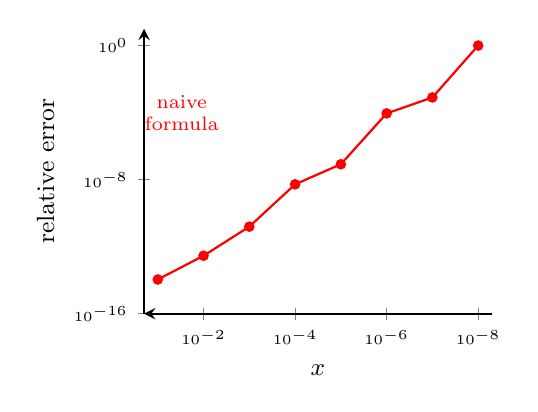
\begin{tikzpicture}
\begin{axis}[width=6cm, height=5.2cm, xmode=log, ymode=log, axis lines=left,
  x dir=reverse, xmin=5e-9, xmax=0.2, ymin=1e-16, ymax=10,
  xlabel={$x$}, ylabel={relative error}, thick,
  tick label style={font=\tiny}, label style={font=\small}]
  \addplot[red, mark=*, mark size=1.5pt] coordinates {(0.1,1.1e-14) (0.01,2.885e-13) (0.001,1.566e-11) (0.0001,5.244e-09) (1e-05,8.275e-08) (1e-06,8.89e-05) (1e-07,0.0007993) (1e-08,1)};
  \node[red, font=\scriptsize, align=center] at (axis cs:3e-2,1e-4) {naive\\formula};
\end{axis}
\end{tikzpicture}\\[2pt]
\scriptsize The smaller $x$, the bigger the error: at $x = 10^{-8}$ the naive formula returns $0$ instead of $0.5$ (100\% error).
\end{column}
\end{columns}
\end{frame}

% ============================================================
\section{Convergence of sequences}
% ============================================================

\begin{frame}{What does ``a sequence converges'' mean?}
\begin{columns}[c]
\begin{column}{0.47\textwidth}
\small
A sequence $x_1, x_2, x_3, \ldots$ \textbf{converges} to $L$ if the error
\[
e_n = |x_n - L|
\]
goes to $0$ as $n \to \infty$.
\begin{block}{Precisely}
For every tolerance $\epsilon > 0$ there is an $N$ such that $|x_n - L| < \epsilon$ for all $n \ge N$.
\end{block}
\small ``Pick any band around $L$; eventually the sequence stays inside it.''
\end{column}
\begin{column}{0.5\textwidth}
\centering
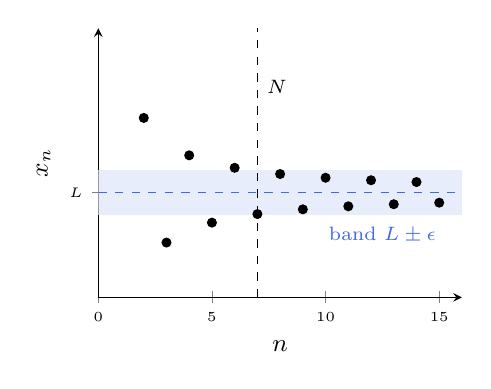
\begin{tikzpicture}
\begin{axis}[width=6.2cm, height=5cm, axis lines=left, xmin=0, xmax=16, ymin=0.3, ymax=2.1,
  xlabel={$n$}, ylabel={$x_n$}, tick label style={font=\tiny}, label style={font=\small},
  ytick={1}, yticklabels={$L$}]
  \fill[accent!12] (axis cs:0,0.85) rectangle (axis cs:16,1.15);
  \draw[accent, dashed] (axis cs:0,1) -- (axis cs:16,1);
  \addplot[only marks, mark=*, mark size=1.6pt, samples at={1,...,15}] {1 + (-1)^x * 1.0/x};
  \draw[dashed] (axis cs:7,0.3) -- (axis cs:7,2.1);
  \node[font=\scriptsize, above right] at (axis cs:7,1.6) {$N$};
  \node[font=\scriptsize, accent] at (axis cs:12.5,0.72) {band $L \pm \epsilon$};
\end{axis}
\end{tikzpicture}\\[2pt]
\scriptsize $x_n = 1 + (-1)^n/n$: from $N$ on, every point stays in the band.
\end{column}
\end{columns}
\end{frame}

\begin{frame}{Three example sequences}
\centering
\small
\begin{tabular}{llll}
\toprule
$n$ & $\left(1+\frac1n\right)^n$ & $x_{n+1} = \cos x_n$ & $x_{n+1} = \frac12\left(x_n + \frac{2}{x_n}\right)$ \\
\midrule
1 & 2.000000 & 1.000000 & 1.000000000000 \\
2 & 2.250000 & 0.540302 & 1.500000000000 \\
3 & 2.370370 & 0.857553 & 1.416666666667 \\
4 & 2.441406 & 0.654290 & 1.414215686275 \\
5 & 2.488320 & 0.793480 & 1.414213562375 \\
\midrule
limit & $e = 2.718281\ldots$ & $0.739085\ldots$ & $\sqrt 2 = 1.414213562373\ldots$ \\
\bottomrule
\end{tabular}

\vspace{0.4cm}
\begin{columns}[T]
\begin{column}{0.32\textwidth}\centering\scriptsize a formula in $n$\\ \textbf{slow}\end{column}
\begin{column}{0.32\textwidth}\centering\scriptsize repeat a function (fixed point)\\ \textbf{steady}\end{column}
\begin{column}{0.32\textwidth}\centering\scriptsize Newton's method for $x^2 = 2$\\ \textbf{very fast}\end{column}
\end{columns}
\vspace{0.3cm}
\begin{block}{Question}
All three converge. How do we measure \emph{how fast}?
\end{block}
\end{frame}

\begin{frame}{Rates of convergence}
\small
Compare each error with the previous one:
\begin{center}
\footnotesize
\begin{tabular}{lll}
\toprule
name & rule & example \\
\midrule
sublinear & $e_n \approx C/n$ & $(1+\frac1n)^n$: \ $e_n = O(1/n)$ \\
linear & $e_{n+1} \approx \rho\, e_n$, \ $0<\rho<1$ & $\cos$ iteration, $\rho \approx 0.67$ \\
quadratic & $e_{n+1} \approx C\, e_n^{2}$ & Newton's method: digits \textbf{double} \\
\bottomrule
\end{tabular}
\end{center}

\begin{columns}[T]
\begin{column}{0.48\textwidth}
\begin{block}{Linear}
Error shrinks by the same factor $\rho$ every iteration: $e_n = O(\rho^{\,n})$.
With $\rho = 0.67$ we gain one digit about every 6 iterations.
\end{block}
\end{column}
\begin{column}{0.48\textwidth}
\begin{block}{Quadratic}
$e_n \approx 10^{-3} \Rightarrow e_{n+1} \approx 10^{-6} \Rightarrow 10^{-12}$.
Newton for $\sqrt2$: errors $2\!\times\!10^{-3},\ 2\!\times\!10^{-6},\ 2\!\times\!10^{-12}$.
\end{block}
\end{column}
\end{columns}
\end{frame}

\begin{frame}{Seeing the rate: plot the error on a log scale}
\begin{columns}[c]
\begin{column}{0.42\textwidth}
\small
Plot $e_n$ with \texttt{plt.semilogy}:
\begin{itemize}
  \item \textbf{linear}: a straight line (slope $\log\rho$);
  \item \textbf{quadratic}: bends down, steeper and steeper;
  \item \textbf{sublinear}: flattens out.
\end{itemize}
\vspace{0.2cm}
\begin{alertblock}{The floor}
Newton reaches $\approx 10^{-16}$ in 5 iterations and cannot go lower: that is machine epsilon.
\end{alertblock}
\end{column}
\begin{column}{0.56\textwidth}
\centering
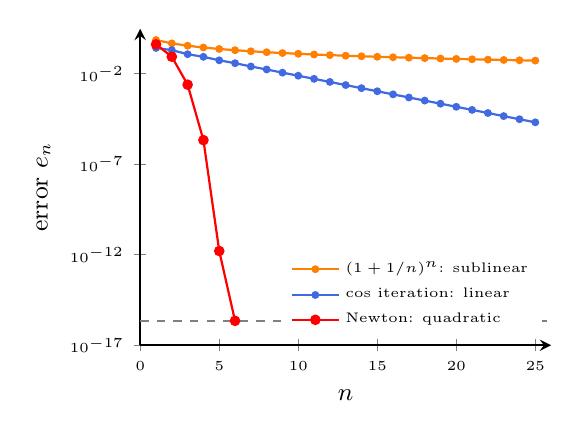
\begin{tikzpicture}
\begin{axis}[width=6.8cm, height=5.6cm, ymode=log, axis lines=left,
  xmin=0, xmax=26, ymin=1e-17, ymax=3, xlabel={$n$}, ylabel={error $e_n$},
  thick, tick label style={font=\tiny}, label style={font=\small},
  legend style={font=\tiny, draw=none, at={(0.98,0.02)}, anchor=south east}]
  \addplot[orange, mark=*, mark size=1pt] coordinates {(1,0.7183) (2,0.4683) (3,0.3479) (4,0.2769) (5,0.23) (6,0.1967) (7,0.1718) (8,0.1525) (9,0.1371) (10,0.1245) (11,0.1141) (12,0.1052) (13,0.09768) (14,0.09113) (15,0.0854) (16,0.08035) (17,0.07587) (18,0.07186) (19,0.06825) (20,0.06498) (21,0.06202) (22,0.05931) (23,0.05683) (24,0.05455) (25,0.05245)};
  \addlegendentry{$(1+1/n)^n$: sublinear}
  \addplot[accent, mark=*, mark size=1pt] coordinates {(1,0.2609) (2,0.1988) (3,0.1185) (4,0.0848) (5,0.0544) (6,0.03772) (7,0.02487) (8,0.01698) (9,0.01133) (10,0.007681) (11,0.005152) (12,0.00348) (13,0.00234) (14,0.001578) (15,0.001062) (16,0.0007159) (17,0.0004821) (18,0.0003248) (19,0.0002188) (20,0.0001474) (21,9.927e-05) (22,6.687e-05) (23,4.504e-05) (24,3.034e-05) (25,2.044e-05)};
  \addlegendentry{$\cos$ iteration: linear}
  \addplot[red, mark=*, mark size=1.5pt] coordinates {(1,0.4142) (2,0.08579) (3,0.002453) (4,2.124e-06) (5,1.595e-12) (6,2.22e-16)};
  \addlegendentry{Newton: quadratic}
  \draw[gray, dashed] (axis cs:0,2.2e-16) -- (axis cs:26,2.2e-16);
  \node[gray, font=\tiny, above] at (axis cs:20,2.2e-16) {machine epsilon};
\end{axis}
\end{tikzpicture}
\end{column}
\end{columns}
\end{frame}

\begin{frame}{Estimating the order from data}
\small
If $e_{n+1} \approx C\,e_n^{\,p}$, then $p$ is the \textbf{order} of convergence ($p=1$ linear, $p=2$ quadratic). From three consecutive errors:
\[
p \;\approx\; \frac{\log\left(e_{n+1}/e_n\right)}{\log\left(e_n/e_{n-1}\right)}
\]
\begin{columns}[T]
\begin{column}{0.5\textwidth}
\begin{exampleblock}{Newton for $\sqrt 2$}
errors: $8.6\!\times\!10^{-2},\ 2.5\!\times\!10^{-3},\ 2.1\!\times\!10^{-6},\ 1.6\!\times\!10^{-12}$\\[3pt]
estimates of $p$: $1.98,\ 2.00$ \ $\Rightarrow$ quadratic.
\end{exampleblock}
\end{column}
\begin{column}{0.46\textwidth}
\begin{block}{Linear: estimate $\rho$}
$\rho \approx e_{n+1}/e_n$.\\
$\cos$ iteration: $\rho \approx 0.67 = |\sin(0.739)|$.
\end{block}
\end{column}
\end{columns}
\vspace{0.2cm}
\scriptsize Use errors that are well above $10^{-16}$: near the floor the estimates become noise.
\end{frame}

\begin{frame}{When floating point meets convergence}
\begin{columns}[T]
\begin{column}{0.5\textwidth}
\small
In exact arithmetic $(1+\frac1n)^n \to e$. On a computer:
\begin{center}
\begin{tabular}{rl}
\toprule
$n$ & computed $(1+\frac1n)^n$ \\
\midrule
$10^{6}$  & 2.7182804690 \\
$10^{8}$  & 2.7182817983 \\
$10^{12}$ & 2.7185234960 \\
$10^{15}$ & 3.0350352065 \\
$10^{16}$ & \cbox{red!20}{1.0000000000} \\
\midrule
$e$ & 2.7182818284 \\
\bottomrule
\end{tabular}
\end{center}
\scriptsize At $n = 10^{16}$, $1 + 10^{-16}$ rounds to exactly $1$.
\end{column}
\begin{column}{0.47\textwidth}
\begin{alertblock}{Lesson}
\small ``$n \to \infty$'' is a mathematical idea. On a computer, rounding error eventually wins.
\end{alertblock}
\begin{block}{Stopping an iteration}
\small Stop when the change per iteration gets small:
\[
|x_{n+1} - x_n| < \text{tol}
\]
and choose tol well above $10^{-16}\,|x_n|$. Always add a maximum number of iterations.
\end{block}
\end{column}
\end{columns}
\end{frame}

% ============================================================
\section{Summary and practice}
% ============================================================

\begin{frame}{Summary}
\begin{columns}[T]
\begin{column}{0.33\textwidth}
\begin{block}{Complexity}
\scriptsize
\begin{itemize}
  \item time = flops, space = memory
  \item $O$ upper bound; $\Omega$ lower, $\Theta$ tight
  \item drop constants and small terms
\end{itemize}
\end{block}
\end{column}
\begin{column}{0.33\textwidth}
\begin{block}{Floating point}
\scriptsize
\begin{itemize}
  \item scientific notation in base 2
  \item 64 bits, about 16 digits
  \item $\varepsilon \approx 2.2\times10^{-16}$
  \item compare with a tolerance
  \item avoid subtracting nearly equal numbers
\end{itemize}
\end{block}
\end{column}
\begin{column}{0.33\textwidth}
\begin{block}{Convergence}
\scriptsize
\begin{itemize}
  \item $e_n = |x_n - L| \to 0$
  \item sublinear, linear, quadratic
  \item \texttt{semilogy} shows the rate
  \item floor at $\approx 10^{-16}$
\end{itemize}
\end{block}
\end{column}
\end{columns}
\vspace{0.4cm}
\centering
\small Big-$O$ connects them: cost $= O(n^2)$, \ error $= O(1/n)$, \ error $= O(\rho^n)$.
\end{frame}



\end{document}
